%% Copyright (C) 2012, Gostai S.A.S.
%%
%% This software is provided "as is" without warranty of any kind,
%% either expressed or implied, including but not limited to the
%% implied warranties of fitness for a particular purpose.
%%
%% See the LICENSE file for more information.

\chapter{MORSE}
\label{sec:morse}

This chapter documents the use of MORSE in the MORSE simulation
environment.

\section{Installation and Setup}

This section describes how to setup the software on your computer and gives
you the basics to use MORSE.  The setup process depends on your OS, please
follow the corresponding instructions.

\subsection{GNU/Linux}

\subsubsection{MORSE installation}

MORSE is available on a git repository.

\begin{shell}
$ git clone http://github.com/laas/morse.git
\end{shell}

You can also get the latest stable version with a tarball at
\href{https://github.com/laas/morse/tarball/0.4}
{https://github.com/laas/morse/tarball/0.4}.

The third solution is to use a package manager to get MORSE.  Every
installation is detailed on the MORSE website
(\href{http://www.openrobots.org/morse/doc/latest/user/installation.html}
{MORSE installation}) and have a look at the FAQ
\href{http://www.openrobots.org/morse/doc/latest/user/faq.html} {MORSE FAQ}.

The first solution is strongly advise since we want to use correctly the
MORSE-ROS binding. See the FAQ section. %FIXME: do a FAQ section.

\subsubsection{Blender installation}

MORSE requires a Blender 2.59 build with Python 3.2.

First, you need to install Blender. Every step of the installation can be found
at \href{http://doc.ubuntu-fr.org/blender_compilation}{Blender compilation}.

You can download Python 3.2 using your package manager.

\begin{shell}
$ sudo apt-get install python3.2
\end{shell}

If you want to build Python, follow this tutorial
\href{http://wiki.blender.org/index.php/Dev:2.5/Doc/Building_Blender/Linux/Troubleshooting}
{Python building}.  Make sure to do the user-config.py at the root directory
of Blender to build it with the Python3.2 version.

If everything has been done correctly, this command should to the following.
\begin{shell}
$ morse check
* Checking up your environment...


* Running on Linux. Alright.

* Found MORSE libraries in '/usr/local/lib/python3.2/site-packages/morse/blender'. Alright.

* Trying to figure out a prefix from the script location...

* Default scene found. The prefix seems ok. Using it.

* Setting $MORSE_ROOT environment variable to default prefix [/usr/local/]

* Checking version of /home/gostai/install/linux/blender... Found v.2.60.0

* Blender found from $MORSE_BLENDER. Using it (Blender v.2.60.0)

* Checking version of Python within Blender /home/gostai/install/linux/blender... Found v.3.2

* Blender is using Python 3.2. Alright.

* Your environment is correctly setup to run MORSE.
\end{shell}

\subsubsection{ROS installation}

MORSE supports middlewares such as MOOS, Pocolibs, ROS, Sockets, Text
middleware and YARP. \urbi has a ROS bridge to communicate with ROS world in
\us.

Two versions of ROS are supported for MORSE.
\begin{itemize}
  \item ROS Diamondback
  \item ROS Electric Emys
\end{itemize}

ROS Electric Emys is strongly advised to avoid any complication but if you
really want to use Diamondback you will have more details about the
workaround to use it.
\href{http://www.openrobots.org/morse/doc/latest/user/installation/mw/ros.html}
{MORSE-ROS installation}

A lot of stacks are needed for MORSE:
\begin{itemize}
\item morse-ros \href{git clone http://code.in.tum.de/git/morse-ros.git}
  {morse-ros repository}
\item ros-electric-roslisp-common
\item nav\_pcontroller
  \href{http://www.ros.org/browse/details.php?name=nav\_pcontroller}
  {nav\_pcontroller stack}
\end{itemize}

Checkout the tutorials branch for morse-ros stack.
\begin{shell}
$ git checkout -b tutorials origin/tutorials
\end{shell}

\paragraph{Script for installation} there is a script made by Pierrick Koch to
install all you need for MORSE-ROS.
(\href{https://github.com/pierriko/proteus/blob/master/morse-ros.sh}{Link})
\subsection{Osx}

The process is exactly the same for Mac OS X. Make sure your Python version
is the expected one and your environment is well set (e.g.,
\env{MORSE\_BLENDER}, \env{PYTHONPATH}).

\subsection{Windows}

MORSE has never been tested on Windows. No documentation is available for it.

\section{Introduction to MORSE-\urbi}

This section will show you how to use MORSE using \urbi to
control the simulation.

The purpose of MORSE is to build, thanks to Blender, a robot with different
components that send or receive information. These are represented in
different middlewares such as ROS.

The following example is based on a MORSE tutorial
(\href{http://www.openrobots.org/morse/doc/latest/user/tutorial.html} {MORSE
  tutorial}) adapted for ROS.

{\cxxPre%
\lstinputlisting[language=Python,style=UrbiSDKEnv,firstline=11]
  {\absTopSrcdir/share/morse/test-ros.py}%
\cxxPost}

Every details about the components can be found here
\href{http://www.openrobots.org/morse/doc/latest/components_library.html}
{components description}.

\section{Run the simulation}

Now we will run the example to test MORSE-\urbi.

Make sure your example is in
\file{my\_morse\_root/examples/morse/scenarii}.

\begin{shell}
$ morse exec test-ros.py
\end{shell}
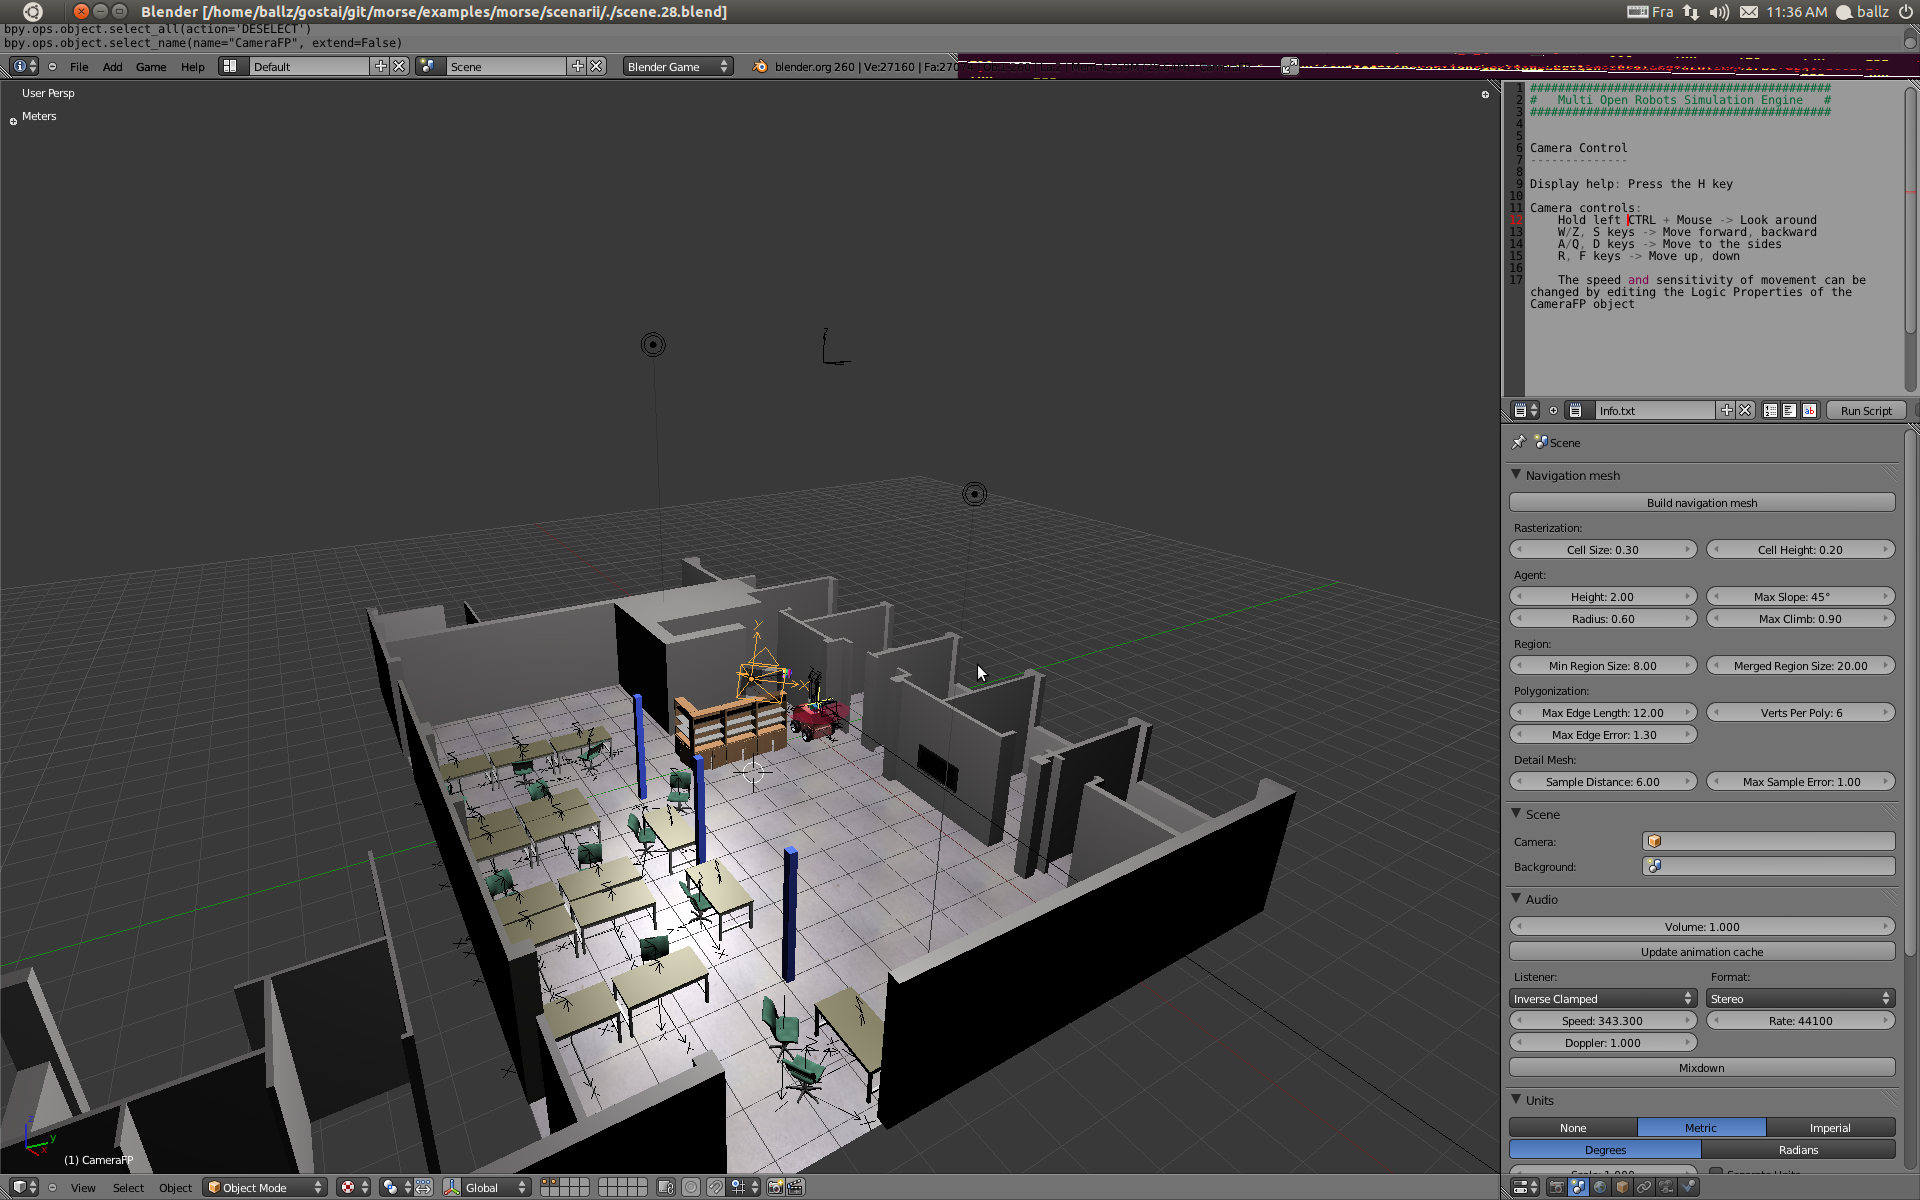
\includegraphics[width=0.95\textwidth]{img/morse/simulation.png}

To run the simulation, press \samp{p}.  Since we bound MORSE using the ROS
middleware, you need have a roscore running.  Otherwise you will have an
error message:
\begin{shell}
Unable to register with master node [http://localhost:11311]: \
master may not be running yet. Will keep trying.
\end{shell}

\begin{shell}
$ roscore
\end{shell}

Now, MORSE will communicate with ROS.

\section{Using \urbi to play with the simulation}

We have several ROS topics that are running.

\begin{shell}
$ rxgraph
\end{shell}

You should have something like this.

\begin{figure}[htp]
  \centering
  \includegraphics[width=0.9\linewidth]{img/morse/rxgraph}
  \caption{Output from \command{rxgraph}}
  \label{fig:morse:rxgraph}
\end{figure}

There is one Publisher and six Subscribers available.

\paragraph{Motion Controller}

With the motion controller publisher, you can change the angular and linear
speed of the Robot and make it move.

\begin{urbiunchecked}
var mv = Morse.MotionControllerSensor |;
mc.changeLinear(1, 1, 1);
mc.changeAngular(1, 1, 1);
mc.move;
// The Robot is now moving.
\end{urbiunchecked}

\paragraph{GPS}

The GPS sensor will give the coordinates of the sensor on the Robot.  The
coordinates provided by the GPS are with respect to the origin of the
Blender coordinate reference.

\begin{urbiunchecked}
var g = Morse.GpsSensor.new |;
g.data;
[00668250] "0.10133811086416245, -0.07535230368375778, 0.7684202194213867, "
\end{urbiunchecked}

\paragraph{CameraMain}

The camera sensor will give the video flow received by the camera set on the
Robot.

Please run a \urbi server to allow \command{urbi-image} to display
camera's content.

\begin{shell}
$ urbi -H 127.0.0.1 -P 54000
\end{shell}

\begin{urbiunchecked}
var vc = Morse.VideoCameraSensor.new |;
vc.run;
\end{urbiunchecked}

Simply run \command{urbi-image} to view through the camera.
\begin{shell}
$ urbi-image
\end{shell}

\paragraph{Pose}

The Pose sensor provides the absolute position and orientation. Do the same
job as GPS.

\begin{urbiunchecked}
var ps = Morse.PoseSensor.new |;
ps.angularPosition;
[00000001] ["x" => -4.6432e-12, "y" => 7.52752e-13, "z" => -4.01468e-12]
ps.linearPosition;
[00000002] ["x" => 3.14342e-09, "y" => 0, "z" => 0]
\end{urbiunchecked}

\paragraph{Odometry}

The Odometry sensor produces relative displacement.

\begin{urbiunchecked}
var o = Morse.OdometrySensor.new |;
ps.angularPosition;
[00000001] ["x" => -7.8332e-12, "y" => 9.62747e-13, "z" => 4.01468e-12]
ps.linearPosition;
[00000002] ["x" => 0, "y" => 0, "z" => 0]
\end{urbiunchecked}

\paragraph{Sick}

The Sick sensor emulates a laser range scanner, by generating a series of
rays in predefined directions, and then computing whether they find any
object within a certain distance of the sensor’s origin.

\begin{urbiunchecked}
var s = Morse.SickSensor.new |;
s.angleMin;
[00000021] -1.5708
s.angleMax;
[00000002] 1.5708
s.rangeMin;
[00000003] 0.3
s.rangeMax;
[00000004] 5
s.ranges |;
\end{urbiunchecked}

\paragraph{Accelerometer}

The Accelerometer sensor emulates an Accelerometer/Pedometer, measuring the
distance that a robot has moved, the current speed and current
acceleration. Measurements are done for the 3 axes (X, Y, Z) for velocity
and acceleration.

\begin{urbiunchecked}
var a = Morse.Accelerometer.new |;
a.data;
[:][00000001] "9.536815923361088e-07, [5.7220458984375e-05, 0.0, -2.2351741790771484e-07], \
[:]                                   [-0.0034332275390625, 0.0, -1.341104507446289e-05], "
\end{urbiunchecked}

%%% Local Variables:
%%% coding: utf-8
%%% mode: latex
%%% TeX-master: "../urbi-sdk"
%%% ispell-dictionary: "american"
%%% ispell-personal-dictionary: "../urbi.dict"
%%% fill-column: 76
%%% End:
